% Kapitel 3

\chapter{Data Efficiency via Model-Driven Preprocessing}
\label{chap:model-driven-preprocessing}

In this chapter, we will propose another way of achieving data efficiency in neural network-based medical image segmentation. Our approach centers on preprocessing the input data using domain knowledge and traditional image-processing techniques to make the image more easily segmentable. However, instead of manually selecting transformation parameters, we will model the parameters as functions of the image, and train a neural network to estimate optimal transformation parameters. As discussed in the previous chapter, regularization enables a network to limit its number of parameters to what is necessary for the given problem's complexity. Through strategic image transformation, we aim to simplify the complexity of the segmentation task, thus allowing for efficient segmentation with fewer parameters.

 We will first present some motivation to show how it is possible to transform data to be easier to model. This is followed by a detailed outline of our method, as well as an empirical study, demonstrating the effectiveness of our approach across various medical image segmentation tasks. We then show an improvement of the method to support multiple segmenting objects and another empirical study using the improved approach.

\section{Motivation: Using The Polar Transform for Preprocessing}

Our approach is centered on discovering transformations of data that enable neural networks to approximate decision boundaries with fewer parameters. This strategy is grounded in a particular interpretation of neural networks. Consider a network tasked with classifying a given image region \(I(x, y)\) as class ``0'' or ``1''. All conceivable image regions \(I(x, y)\) form part of a \(d\)-dimensional space, known as the input space. Here, \(d\) represents the total number of pixels in the region multiplied by the number of channels in each pixel. The neural network, through iterative optimization, seeks to transform the input space into some other $n$-dimensional in such a way that it becomes linearly separable by an $n$-dimensional hyperplane into two distinct classes. This process and its outcome are depicted in \figref{fig:input-space-transform}.

	\begin{figure}[t!]
		\centering
		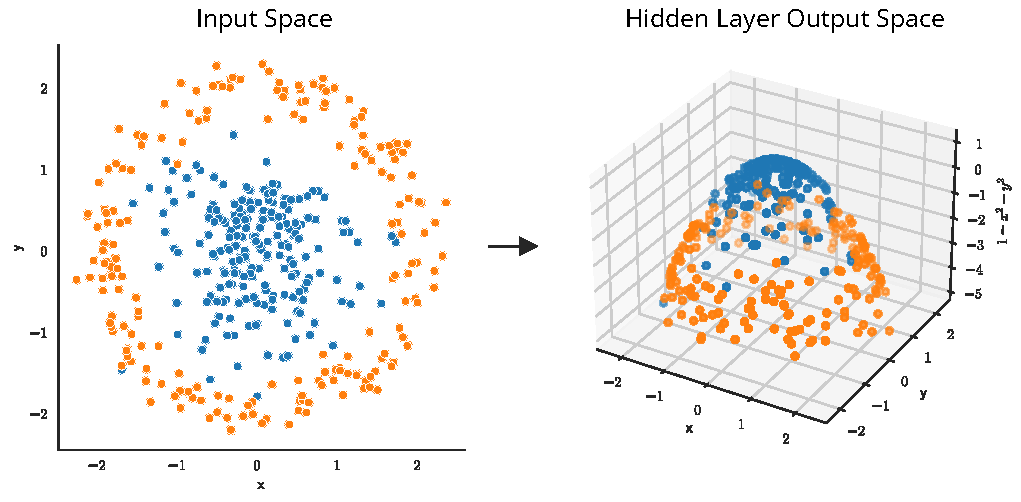
\includegraphics[width=0.65\linewidth]{images/4/nn_trans_dataset}
		\caption{An example of how a 2-class classification neural network bends an input space (left) such that it is linearly separable with a hyperplane.}
		\label{fig:input-space-transform}
	\end{figure}

To find the transformation, the network needs a sufficient number of parameters. More parameters allow for more complex transformations. For instance, to accurately approximate a circular decision boundary, the network needs at least three neurons in its second layer. We exemplify this in \figref{fig:circ-datataset-neurons}.

	\begin{figure}[t!]
		\centering
		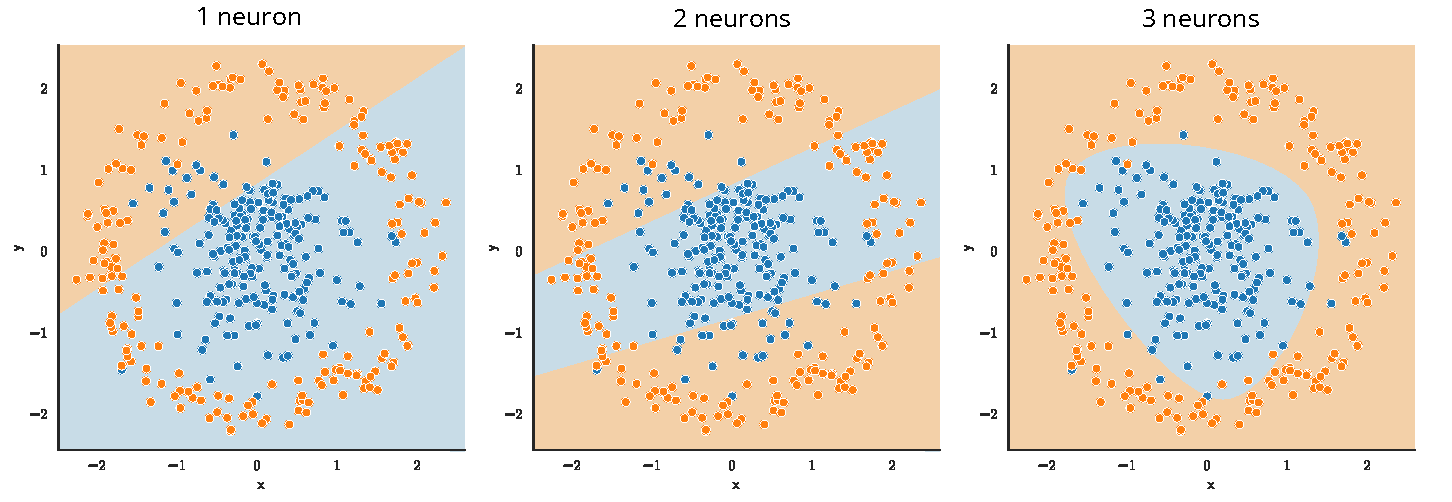
\includegraphics[width=\linewidth]{images/4/circular_dataset_neurons}
		\caption{The decision boundary (shown as the background color) according to a fully connected neural network with three layers where the second layer has one, two, or three neurons.}
		\label{fig:circ-datataset-neurons}
	\end{figure}

% The essence of data efficiency in neural networks is to establish a decision boundary using fewer data samples. This is achieved by narrowing the search space of the function class or, in simpler terms, reducing the number of parameters within the neural network. In the current and subsequent chapters, our focus will be on devising methods to pre-process the data into an intermediary form, denoted as \(\mathcal{X}_{pre}\), which is more easily separable than the original input space \(\mathcal{X}\). By transforming data into \(\mathcal{X}_{pre}\), which is closer to the ideal transformed space \(X'\), the network requires fewer parameters as it has a smaller search space to find \(X'\). This transformation process is referred to as \(\mathcal{T}\).

% A prime example of such a transformation is the polar transform. Specifically in two dimensions, the polar transform \(\mathcal{T}(X_i; C)\), defined by a chosen origin \(C = [c_0, c_1]\), converts an input vector \(X = [x_0, x_1]\) into a vector \(\mathcal{T}_C(X) = [\theta, r]\). The transformation is as follows:

The goal of data efficiency is to find a decision boundary given fewer data samples. As discussed in the previous chapter, this necessitates narrowing the search space of possible decision boundaries, or, in other words, reducing the number of neural network parameters. In the current and subsequent chapters, our focus will be on devising methods to pre-process the data into an intermediary form, denoted as \(\mathcal{X}_{pre}\), which is more easily separable than the original input space \(\mathcal{X}\). By transforming data into \(\mathcal{X}_{pre}\), the network requires fewer parameters as it has a smaller search space to find \(X'\). This transformation process is referred to as \(\mathcal{T}\).

A commonly used example of $\mathcal{T}$ is the polar transform. In the two-dimensional case, the polar transform \(\mathcal{T}(X_i; C)\), defined by a chosen origin \(C = [c_0, c_1]\), converts an input vector \(X = [x_0, x_1]\) into a vector \(\mathcal{T}_C(X) = [\theta, r]\). The transformation is as follows:
\begin{equation}
    \begin{aligned}
	r =& \sqrt{(x_0 - c_0)^2 + (x_1 - c_1)^2},\\
	\theta =& arctan(x_1 - c_1, x_0 - c_0)
    \end{aligned},
\end{equation}
where $arctan(x, y)$ is the two-argument arcus tangent function, defined as the angle between the vector $(x, y) \in \mathbb{R}^2 \backslash\{0\}$ and the positive x-axis.

The polar transform effectively converts a circular decision boundary into a linear one. This transformation enables linear separability in our example dataset, which then requires only a single neuron in the second layer for effective classification. This is demonstrated in \figref{fig:polar_dataset_neurons}.

	\begin{figure}[t!]
		\centering
		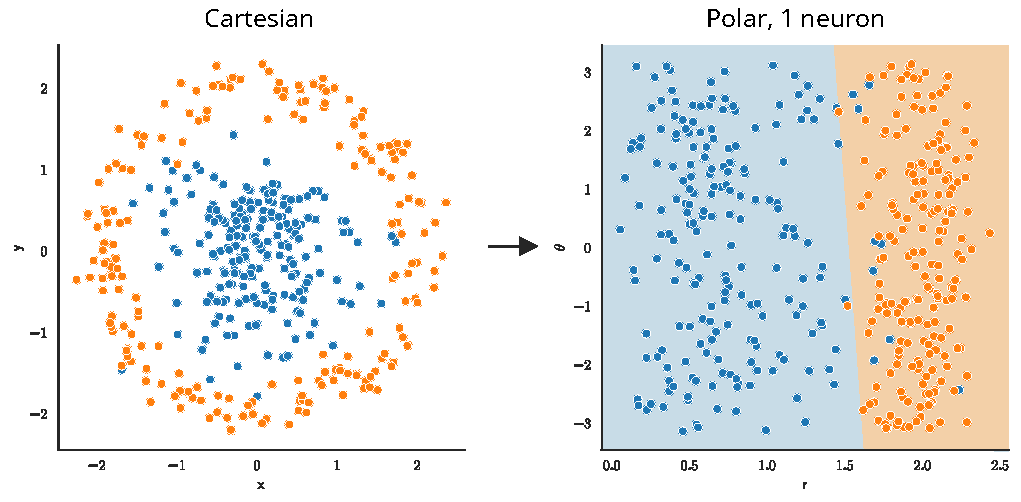
\includegraphics[width=0.65\linewidth]{images/4/polar_dataset_neurons}
		\caption{An example circular dataset transformed using the polar transform. The background color shows the decision boundary of a fully connected network with one neuron in the second layer.}
		\label{fig:polar_dataset_neurons}
	\end{figure}
	
However, the key to the polar transform's success in facilitating separability lies in the correct selection of the polar origin. When the origin is shifted away from the center of class ``0'', the decision boundary in the polar space ceases to be linear. This effect of origin displacement on the linearity of the decision boundary in the polar space is illustrated in \figref{fig:polar-origin-selection}.

 	\begin{figure}[t!]
		\centering
		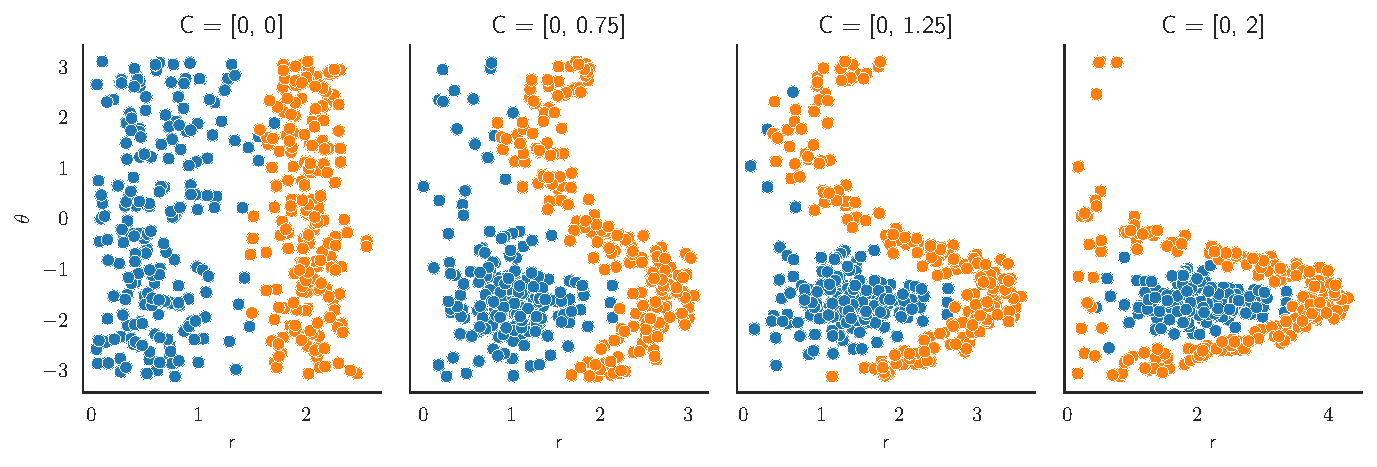
\includegraphics[width=\linewidth]{images/4/data_polar_origin}
		\caption{The polar transformation of the simulated data using different polar origins ($C$).}
		\label{fig:polar-origin-selection}
	\end{figure}
	
	Building on the example of the polar transform, we propose a methodology where key transformation parameters, like the polar origin, are dynamically estimated using a neural network. We call this approach model-driven preprocessing, specifically tailored to enhance data efficiency in medical image segmentation.
	
\section{Model-driven Preprocessing}

The concept illustrated with the polar transform can be effectively applied to image segmentation. Imagine an image where pixels belonging to one class form a circular pattern, with the background occupying the space outside this circle. A segmentation model tasked with this scenario needs to approximate a circular boundary to segment the image accurately. By applying the polar transform, this circular boundary is converted into a linear one, significantly simplifying the task and allowing for segmentation with a less complex model.

We propose a general formulation of this approach, wherein images are transformed to be more linearly separable using carefully selected transformations derived from traditional image processing methods. The success of these transformations hinges on the correct selection of parameters. To address this, we employ neural networks trained specifically to predict these optimal transformation parameters. The preprocessed image is then segmented using a regular neural network. Importantly, since the preprocessed image is inherently simpler to segment, the segmentation network can be designed with fewer parameters compared to a network segmenting unprocessed images. This is, in essence, a model-driven approach to preprocessing the image. A visual summary of this approach is shown in \figref{fig:visual-summary-mdp}. In the remainder of this section, we will describe this approach in more detail.

 	\begin{figure}[t!]
		\centering
		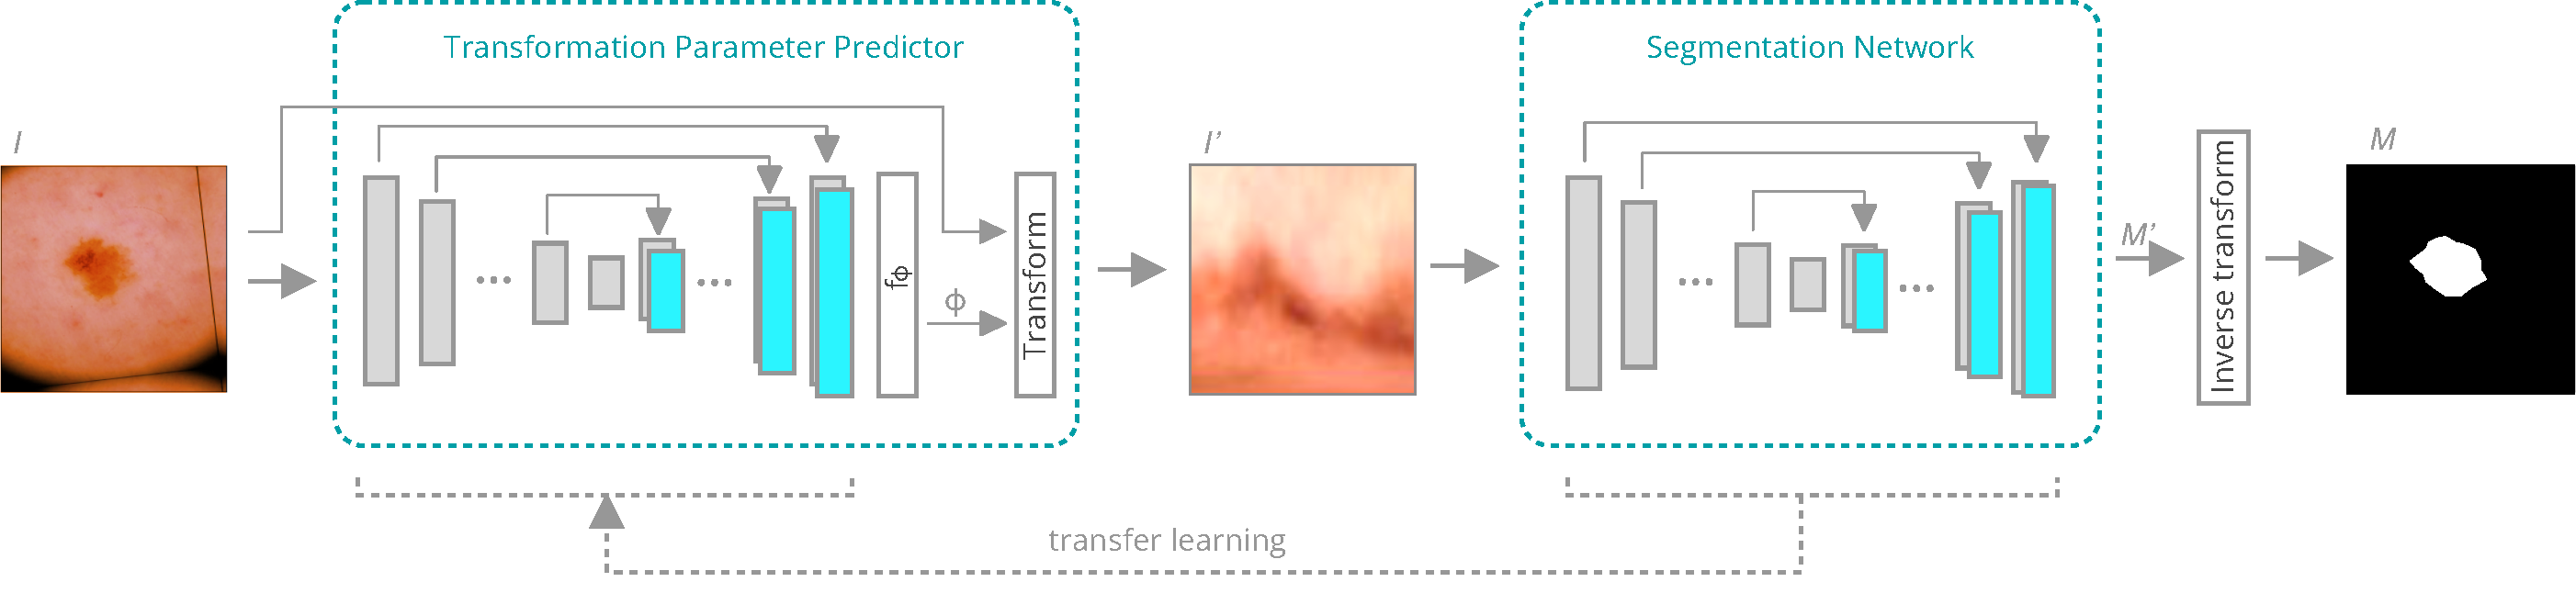
\includegraphics[width=\linewidth]{images/4/model-based-preprocessing-overview}
		\caption{A visual summary of the model-driven preprocessing approach. First, the transformation parameter predictor network predicts a segmentation-like map, from which the transformation parameters are calculated using a transformation parameter function. Then, the input image is transformed and the transformed representation is segmented by a segmentation neural network. The final segmentation map is obtained by inverting the transformation.}
		\label{fig:visual-summary-mdp}
	\end{figure}

To preprocess the image, we select a transformation function \(\mathcal{T}_{\phi}(I)\), where \(\phi\) represents the transformation parameters, and \(I\) is the original image. This transformation yields a new image, \(I'\), which can be segmented with fewer parameters than the original. 

The transformation function \(\mathcal{T}\) can vary, encompassing affine transformations, deformation fields, thresholding techniques, and, as previously mentioned, the polar transform. The choice of \(\mathcal{T}\) is contingent upon the specific segmentation task. For instance, the polar transform is advantageous for segmenting elliptical objects. When segmenting small objects, we might opt for an affine transformation that scales each object to a uniform scale. The design of \(\mathcal{T}\) should be informed by domain knowledge and validated through empirical testing. An important requirement is that \(\mathcal{T}\) must be invertible, allowing the resulting segmentation mask to be mapped back to the original image space. The segmentation process on the transformed image can be represented as:
\begin{equation}
	M(I) = (\mathcal{T}_{\phi}^{-1} \circ F_{seg} \circ \mathcal{T}_{\phi})(I),
\end{equation}
where $M(I)$ is the resulting segmentation mask for image $I$, $F_{seg}$ is the segmentation neural network. 

The effectiveness of preprocessing is highly dependent on the appropriate choice of \(\phi\), as illustrated with the polar transform. It's also important to note that \(\phi\) is specific to each image: the origin, scale, location, and distribution of objects differ across images. Acknowledging this, we propose training a model to estimate the optimal \(\phi\) for a given image:
\begin{equation}
	\phi(I) = F_{\mathcal{T}}(I; \theta_{\mathcal{T}}),
\end{equation}
where $F_{\mathcal{T}}$ is a neural network with parameters $\theta_{\mathcal{T}}$ trained to estimate the correct parameters for $\mathcal{T}$ given an image $I$. In our approach, we use various types of neural networks as $F_{\mathcal{T}}$, though it is also possible to use more traditional approaches.

More precisely, $F_{\mathcal{T}}$ is structured similarly to a regular segmentation network, producing a segmentation mask $M_\phi(I)$ in its second-to-last layer. The final layer, which is a non-trainable function $\phi(I) = f_\phi(M_\phi(I))$, produces segmentation parameters given a predicted segmentation map. $F_{\mathcal{T}}$ can then be expressed as:
\begin{equation}
	F_{\mathcal{T}}(I; \theta_{\mathcal{T}}) = f_\phi(F_{\mathcal{T}seg}(I; \theta_{\mathcal{T}})),
\end{equation}
where $F_{\mathcal{T}seg}$ is the segmentation sub-network producing $M_\phi(I)$. $F_{\mathcal{T}seg}$ can be trained using segmentation-like loss functions, where $M_\phi$ can be compared to a ground truth segmentation mask $M_{gt}(I)$. 

The function $f_\phi$ is hand-constructed using knowledge of the transformation. For instance, we know that for the polar transform, the optimal origin lies in the center of the object. Therefore, we may use the centroid of the ground truth segmentation labels as $f_\phi$. Other examples of \( f_\phi \) for various transformations include:

\begin{itemize}
	\item \textbf{CT Thresholding}: The transformation parameters are the maximum and minimum Hounsfield units representing a specific tissue. The function \( f_\phi \) could use the minimum and maximum values within the predicted segmentation mask to determine these parameters.
	\item \textbf{Rescaling}: For rescaling transformations, the parameters are the \( x \) and \( y \) scaling factors. We can determine these factors using the predicted segmentation mask to ensure that the object attains a predefined fixed width and height.
	\item \textbf{Translation}: The translation parameters, in terms of \( x \) and \( y \) shifts, can be calculated by measuring the distance between the object's center and a desired reference point.
\end{itemize}

It's important to note that \( M_\phi(I) \) doesn't have to be a conventional segmentation mask. Depending on the requirements for predicting optimal transformation parameters, we can create pseudo-labels that are more suitable for the task. For example,
 in cases where transformation parameters are contingent on an object's centroid, \( M_\phi(I) \) could be modeled as a heatmap with its focus on the object's central point. This approach enables the network to learn to predict the centroids of objects rather than their boundaries. Consequently, \( f_\phi \) can determine the object's centroid by locating the pixel with the highest intensity in \( M_\phi(I) \).

Using this approach, data efficiency is achieved by reducing the total function class size when compared to a standard segmentation neural network. We do so by using two smaller neural networks instead of one large one. Since the decision boundaries of the preprocessed images are simplified, the segmentation network needs fewer parameters to model them. Transformation parameters often have a much smaller dimensionality than the segmentation mask, and therefore the network predicting transformation parameters can naturally use much fewer parameters.

The core idea of our approach is that $\mathcal{T}$ will simplify the segmentation problem such that a regularized segmentation network $F_{seg}$ will be able to perform the segmentation using fewer parameters. To effectively implement this, both \(F_{\mathcal{T}}\) (the network predicting transformation parameters) and \(F_{seg}\) (the segmentation network) require specialized training techniques, which will be elaborated in the forthcoming section.

\subsection{Training Model-Driven Preprocessing Networks}

As mentioned earlier, using the approach of model-driven preprocessing requires specific neural network training techniques. In our approach, two separately trained neural networks are used: the transformation parameter predictor $F_{\mathcal{T}}$ and the segmentation network $F_{seg}$. 

\subsubsection{Training the Transformation Parameter Predictor}

\(F_{\mathcal{T}}\) is designed to process original, untransformed images and output the corresponding transformation parameters, \( \phi(I) \). As previously discussed, the penultimate layer of \(F_{\mathcal{T}}\) generates a segmentation-like mask \( M_\phi(I) \). The training data for \(F_{\mathcal{T}}\) comprises pairs of images and their corresponding ground truth masks, represented as \((I, M_{gt})\). Given a predicted segmentation mask $M_\phi = F_{\mathcal{T}seg}(I)$ and the transformation parameter function $f_\phi(M(I))$, the transformation parameters loss $L_\mathcal{T}$ can be calculated as:
\begin{equation}
	L_\mathcal{T}(I, M_\phi, M_{gt}) = \alpha L_\phi(f_\phi(M), f_\phi(M_{gt})) + \beta L_{M}(M_\phi, M_{gt}),
\end{equation}
where $L_\phi$ measures the error in predicting the transformation parameters, while $L_{M}$ is a segmentation-like loss that measures the error in predicting the segmentation mask used to calculate the transformation parameters. The coefficients \(\alpha\) and \(\beta\), which balance these two terms, are determined empirically.

\subsubsection{Training the Segmentation Network}

The segmentation network is trained using ground-truth transformation parameters (\(\phi\)) to preprocess the input image. For every pair of image and ground truth segmentation label \((I, M_{gt})\), the ground truth transformation parameters are derived using:
\begin{equation}
	\phi = f_\phi(M_{gt}) + z_\phi,
\end{equation}
where \(f_\phi\) is the transformation parameter function, identical to the one used in the parameter predictor network. The term \(z_\phi\) represents a random noise vector matching \(\phi\)'s dimensions. This noise serves as a form of augmentation, enhancing the segmentation network's resilience to less-than-ideal \(\phi\) predictions.

Given $\phi$, the input to the segmentation network is constructed as $I' = \mathcal{T}_\phi(I)$. The network's final layer applies an inverse transformation to the output segmentation map, \(\mathcal{T}^{-1}_\phi(M)\). To train the network, we use a standard segmentation loss $L_{seg}(M, M_{gt})$.

\subsubsection{Transfer Learning}

Given that the parameter predictor mirrors the structure of a segmentation network, we can utilize the same encoder and decoder in both networks, leveraging various forms of transfer learning. This approach offers several advantages:

\begin{enumerate}
	\item Both networks employ a standard encoder, enabling the initialization of these networks with weights pre-trained on extensive medical or natural image datasets.
	\item The development process can start by training a standard baseline segmentation model on untransformed data. Subsequently, the learned weights from this model can be transferred to both the segmentation and transformation parameter predictor networks. In this case, the parameter predictor already knows how to localize the objects, thereby enhancing its ability to predict optimal transformation parameters.
	\item The transformation parameter predictor network's main role is to robustly transform input images. Domain shifts or unrealistic data, which are critical concerns for the segmentation network, are less problematic for the parameter predictor. This leniency allows for the use of extensive augmentation during training, further improving the network's robustness and adaptability.
\end{enumerate}

Having laid out the theoretical framework of this approach, the remainder of this chapter will detail a specific application of this methodology, demonstrated through an empirical study across various medical imaging datasets. This study aims to showcase the practical effectiveness and adaptability of the model-driven preprocessing approach in real-world scenarios.

\section{Model-Driven Polar Transform Using Centerpoint Prediction}
\label{polar-paper}

Earlier in this chapter, we discussed how the polar transform can simplify complex decision boundaries, making segmentation tasks more manageable. Drawing from this insight, this section introduces a practical implementation of our model-driven preprocessing approach, utilizing the polar transform. The approach involves two networks: a transformation parameter predictor and a segmentation network. In this specific implementation, the parameter predictor is designed to determine the polar origin of an image, functioning as a centerpoint predictor network. Its objective is to identify the center of a singular object within the image. We will explore two distinct designs for this centerpoint predictor network:

1. \textbf{Segmentation-like Network}: This design focuses on identifying the centroid of a segmentation mask. It operates like traditional segmentation networks but is specifically optimized to pinpoint the center of an object.

2. \textbf{Heatmap Prediction Network}: Alternatively, this network predicts the centerpoint directly as a heatmap. This approach is more direct, as it aims to localize the object's center without necessarily delineating its entire boundary.

Once the centerpoint is determined, the image undergoes a transformation using the predicted polar origin. The transformed image is then fed into a segmentation network that has been trained on images processed with the polar transform. This setup aims to demonstrate the effectiveness of preprocessing in simplifying the segmentation task, potentially allowing for more accurate and efficient segmentation with neural networks. The subsequent parts of this section will delve into the specifics of these network designs and their performance in practical scenarios.

Our method is evaluated on 
the tasks of polyp segmentation, liver segmentation, skin 
lesion segmentation, and epicardial adipose tissue (EAT) segmentation.
The proposed method can be used as a pre-processing step for 
existing neural network architectures, so we evaluate the methods using
common neural network architectures for medical image segmentation including U-Net 
\cite{ronnebergerUNetConvolutionalNetworks2015}, U-Net++ 
\cite{zhou2019unetplusplus} with a ResNet \cite{heDeepResidualLearning2016} encoder, and DeepLabV3+ \cite{chenEncoderDecoderAtrousSeparable2018} with a ResNet \cite{heDeepResidualLearning2016} encoder. Evaluation of our approach as a pre-processing step shows that it improves segmentation performance across different datasets and neural network architectures while making the networks more robust to small dataset sample sizes.

\subsection{Background and Related Work}

The polar transform's potential for simplifying the segmentation of images with elliptical borders was discussed earlier in this chapter. Transforming such images into polar coordinates effectively turns a perfect circle from Cartesian coordinates into a straight line, significantly simplifying the decision boundary. This simplification means that a less complex model can accurately predict borders in polar coordinates. As illustrated in \figref{fig:polar-lesion}, even for complex shapes, transforming roughly elliptical objects into polar coordinates can reduce the complexity required for accurate segmentation. Moreover, by using the object's center as the polar origin, the approach standardizes the location and border distances in each training example. This standardization allows the model to focus on learning the border distance from the origin at various angles, obviating the need for object localization learning.

	\begin{figure}[t!]
		\centering
		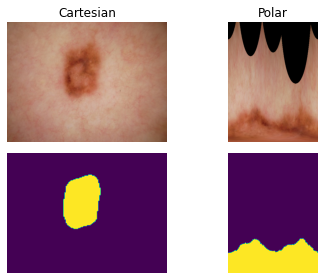
\includegraphics[width=0.4\linewidth]{images/4/to_polar}
		\caption{An example image and label from the lesion dataset and their corresponding polar transformation. \cite{bencevicTrainingPolarImage2021}}
		\label{fig:polar-lesion}
	\end{figure}

Given a polar origin $(c_x, c_y)$ of a Cartesian image $I(x, y)$ of resolution $H \times W$, we obtain each point $(r, \vartheta)$ of the polar transformed image $I'(r, \vartheta)$ as:
  \begin{equation}
    \begin{aligned}
      r &= \frac{H}{2 \pi} \cdot arctan(x, y) [ \cdot 180 / \pi ], \\
      \vartheta &= \frac{W}{\sqrt{(W / 2)^2 + (H / 2)^2}} \cdot \sqrt{x^2 + y^2}
    \end{aligned},
    \label{eq:polar-transform}
  \end{equation}
  where $arctan$ is the 2-argument arctangent function.

    \subsubsection{Previous work using the polar transform for medical image processing}
    
Several image segmentation methods were proposed that utilize polar coordinates. 
\citet{liuDDNetCartesianpolarDualdomain2019a} proposed an approach they
call Cartesian-polar dual-domain network (DDNet) to perform optic disc and cup segmentation
in retinal fundus images. The neural network contains two encoding branches, one for a Cartesian input image and another for the polar transformation of the same input image. The predictions are fused into a single feature vector which is then decoded into a final segmentation.
\citet{salehinejadImageAugmentationUsing2018} used the polar transformation as a way to 
augment
training data by transforming each input image into multiple polar images at various polar
origins, thus increasing the number of training data.
\citet{kimCyCNNRotationInvariant2020a} proposed a convolutional neural network layer for 
images in polar 
coordinates to achieve rotational invariance. Their cylindrical convolution layer uses cylindrically sliding windows to perform a convolution.
\citet{kimCNNBasedUGS2018} proposed a user-guided segmentation method where an expert 
selects the
point used as the polar origin. The transformed image is then
segmented using a convolutional neural network (CNN). 
\citet{estevesPolarTransformerNetworks2018a} proposed a polar transformer network for image 
classification. Note that "transformer network" here refers to spatial transformer networks 
\cite{jaderbergSpatialTransformerNetworks2016} and not attention-based networks commonly called 
transformers.
The network 
consist of a polar origin predictor and a neural network that predicts a heatmap. The centroid of the heatmap is then used as the origin for a polar transformation of the input image. The polar image is classified using a CNN. This approach is most similar to our proposed method, 
however, their approach focuses on image classification, not segmentation. Additionally, our approach differs in the ways the ground truth data is prepared, the neural network architectures, as well as other details.

While there are proposed methods that combine polar transformation with neural networks, most of them solve classification tasks. Some medical image segmentation methods use the polar transformation as a preprocessing step, however, the way they obtain the origin of the polar transformation is usually based on heuristics. To our knowledge, there is currently no work that explores using the polar transformation with a dynamic polar origin as a preprocessing step for semantic segmentation in a variety of medical image datasets.

  \subsection{Methodology}
  
All of the proposed methods rely on training a neural network model to segment polar images. To train on 
polar images, the input images need to be transformed using a polar origin which is near the center of 
the 
segmented object. The correct origin is not known ahead of time, so a prerequisite for predictions on polar
images is a method to determine the correct polar origin. We propose and 
evaluate two different methods for automatically obtaining the polar origin: (1)
estimation via a segmentation trained on non-polar images and (2) training a center-point predictor that predicts heatmaps from input images. 
This section describes these methods, as well as methods to train the 
final segmentation model on the polar images.
      
In each of our approaches, the final segmentation is done using a neural network trained on polar 
transformations of the input images. In the rest of this paper, we refer to this network as the polar 
network. In all of the described approaches, the polar transformation is not part of the network architecture itself, but happens as a preprocessing step for the polar network.
To transform each input image, the polar origin is determined as the center of mass of the 
ground truth label for that image. The center of mass of an image $I(x, y)$ is calculated by first 
calculating the spatial image moments matrix $M$, where the entry of the matrix at row $i$ and column $j$ is calculated as:
  \begin{equation}
    M_{ij}= \sum _{x,y} I(x,y) \cdot x^i \cdot y^j.
    \label{eq:moments}
  \end{equation}
The center of mass $(c_x, c_y)$ of the image can then be calculated as:
  \begin{equation}
    \begin{aligned}
      c_x &= M_{10} / M_{00}, \\
      c_y &= M_{01} / M_{00}
    \end{aligned}.
    \label{eq:center-mass}
  \end{equation}

Finally, to increase the model's robustness to suboptimal center point predictions, we augment the 
calculated center for training images \cite{estevesPolarTransformerNetworks2018a}. Each training image has 
a 30\% chance of varying the center's x and y coordinates by a random value in the range $(-0.05S, 
0.05S)$, where $S$ is the smallest resolution of the image, i.e. $S = min(W, H)$.
 
    \subsection{Centerpoint prediction}
    
Once the polar network is trained, inference can be done by transforming an input image to polar 
coordinates. The polar network requires choosing a center that is close to the center of mass of the 
segmented object. Because a future input image is unlabeled, the correct center needs to be inferred from 
the image. We propose two ways to accomplish this, described in this section.
	
	\pagebreak

	\begin{figure*}[t!]
		\centering
		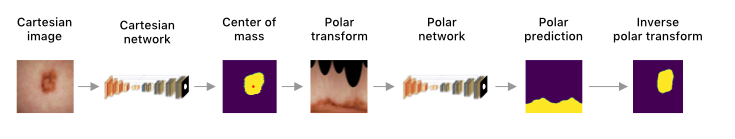
\includegraphics[width=\linewidth]{images/4/retraining-approach}
		\caption{A diagram of the approach (A) of predicting polar origins from a Cartesian network. The first network performs an initial segmentation, which is then used to extract a polar origin for the polar transformation. The method does not rely on any specific neural network architecture. The Polar and Cartesian network can be any neural network that takes an input image and produces a binary segmentation mask as output. The red point shows the extracted polar origin. The Polar network is trained on polar image transformations. The polar transformation is not part of the network itself, but happens as a preprocessing step for the Polar network. \cite{bencevicTrainingPolarImage2021}}
		\label{fig:retraining-diagram}
	\end{figure*}
	
		\begin{figure*}[t!]
		\centering
		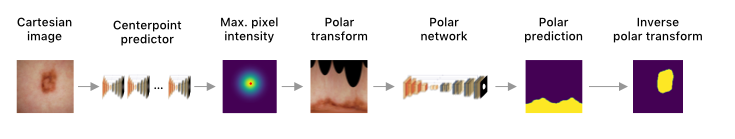
\includegraphics[width=\linewidth]{images/4/centerpoint-approach}
		\caption{A diagram of the approach (B) of using a centerpoint prediction network. The first network can be any neural network that predicts a heatmap from an input image, which is then used to extract the polar origin, shown as a red point. The Polar network can be any semantic segmentation neural network that produces a binary mask output from an input image. The Polar network is trained on polar image transformations. The polar transformation is not part of the network itself, but happens as a preprocessing step for the Polar network. \cite{bencevicTrainingPolarImage2021}}
		\label{fig:centerpoint-approach}
	\end{figure*}

   \subsubsection{(A) Training the same neural network on cartesian and polar images}
   \label{retraining-approach}
   
Our first approach is training the same neural network on cartesian and polar images. A summary of this
approach is presented in \figref{fig:retraining-diagram}. With this approach, 
the inference is done by first feeding the original Cartesian input images into a neural 
network used for segmentation. We refer to this network as the Cartesian network.
For an input image, the polar origin is calculated as the center of mass of the Cartesian network's
prediction for that input image, using \eqref{eq:center-mass}.
This polar origin is used to transform the original input image to polar coordinates, and the transformed 
image is fed
to the polar network. The output of the polar network is transformed back to Cartesian coordinates
to obtain a final segmentation. We assume 
identical architectures for both the Cartesian and polar networks. This makes applying this
framework to existing architectures very straightforward, as it does not require designing new neural 
network architectures or specific hyperparameter optimization and allows for the use of transfer learning to
initialize the networks.
	
    \subsubsection{(B) Training a centerpoint predictor}
    \label{centerpoint-approach}
    
In the second approach for determining the optimal polar origin, we train a model specifically tasked with predicting the correct
polar origin for each input 
image, which is then used to transform the input image. The approach is shown in \figref{fig:centerpoint-approach}. 
We do this by training a neural network based on the stacked hourglass architecture 
\cite{newellStackedHourglassNetworks2016} first used for human pose estimation. Instead of training a regressor network to
predict key points in an image, the stacked hourglass architecture uses a series of stacked encoder-decoder networks, where the output
of each stack is a heatmap centered on the key point to be predicted. The output of each stack is fed as input into the next stack, allowing 
successive refinement of the heatmap prediction. During training, the loss of each stack's output is averaged to produce the final loss, 
allowing deep supervision. The final prediction heatmap is the output of the last stack in the network. To predict the center point, 
we use 8 stacked hourglass blocks, which we empirically determined as the value providing the best results. The network receives images in Cartesian 
coordinates and predicts a heatmap of the image.

\subsubsection{Data Processing}
 
 	\begin{figure}[b!]
		\centering
		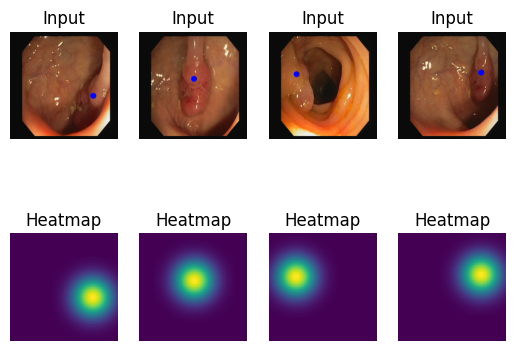
\includegraphics[width=0.8\linewidth]{images/4/heatmaps}
		\caption{Examples of heatmaps generated from the ground truth data. The heatmap is a Gaussian centered on the center of mass of the ground-truth label, shown as a blue point on the input images. \cite{bencevicTrainingPolarImage2021}}
		\label{fig:heatmap}
	\end{figure}
	
The ground truth heatmaps were generated by calculating the center of mass of each ground truth label 
image using \eqref{eq:center-mass}. We then create the heatmap as an image with a 2D Gaussian with the
mean on 
the center of mass on the image and a standard deviation of 8 pixels for all datasets except the liver, and 16 for the liver. The optimal value for the standard deviation was determined empirically on the 
validation datasets. We found that the optimal value of the standard deviation is proportional to the size 
of the object.
Example heatmaps are shown in 
\figref{fig:heatmap}.
	
Additionally, during training, we use augmentation to increase the number of training inputs. In 
particular, during training for each input example, the following random augmentations are applied: (1) a 50\% chance of a horizontal flip; (2)a  30\% chance of a random combination of shifting up to 6.5\% of the image dimensions, scaling up to 10\% and rotating up to 45$^{\circ}$; and (3) a 30\% chance for a grid distortion, details of which are described in \cite{info11020125}.
	
The center-point predictor outputs 8 separate heatmaps \cite{newellStackedHourglassNetworks2016}. We
calculate the predicted center as the coordinates of the pixel with the largest intensity in the heatmap
predicted by the final layer of the model. This predicted center is then used to transform the input
image to polar coordinates, and the transformed image is fed into the polar network to perform
the segmentation. Finally, the segmentation label is transformed back to Cartesian coordinates.
    
  \subsection{Experiments} \label{experiments}
  
To validate the generality of our approach, we trained a variety of neural network architectures on 
multiple medical imaging datasets. In particular, we trained three different neural network 
architectures: U-Net \cite{ronnebergerUNetConvolutionalNetworks2015}, U-Net++ 
\citet{zhouUNetNestedUNet2018} with a ResNet encoder and DeepLabV3+ 
\cite{chenEncoderDecoderAtrousSeparable2018} with a ResNet encoder. Notably, each dataset we use presents a problem wherein almost all examples a single roughly elliptical object needs to be segmented. 
For each dataset and network architecture combination, we train a Cartesian and polar network, and we then 
perform four different experiments: 

\begin{enumerate}
	\item{testing the Cartesian network using Cartesian images}
	\item{testing the polar network using the ground-truth polar origin}
	\item{testing the polar network using polar origins obtained from predictions of the Cartesian network, as outlined in \ref{retraining-approach}}
	\item{testing the polar network using polar origins from the centerpoint predictor, as outlined in \ref{centerpoint-approach}}.
\end{enumerate}

    \subsubsection{Datasets description}

We used four different datasets to train the network. In this section, we give an overview of each used dataset and how it was preprocessed. Note that for training the center-point predictor, the input images were resized to a resolution of $256 \times 256$, while the generated heatmaps were resized to $64 \times 64$ pixels. Otherwise, all preprocessing steps described here are applied to the center-point model datasets as well. Each dataset was normalized and zero-centered to facilitate better network convergence. 

	\begin{figure*}[t!]
	\subfloat[Polyp dataset]{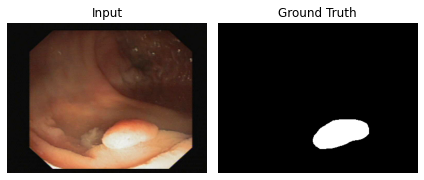
\includegraphics[width=0.49\columnwidth]{images/4/polyp_example}}
	\hfill
	\subfloat[Lesion dataset]{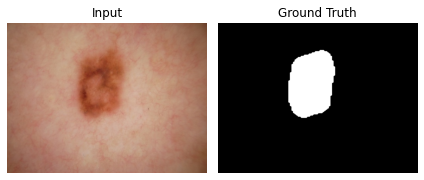
\includegraphics[width=0.49\columnwidth]{images/4/lesion_example}} \\
	\subfloat[Liver dataset]{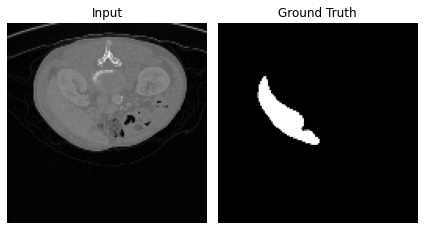
\includegraphics[width=0.49\columnwidth]{images/4/liver_example}}
	\hfill
	\subfloat[EAT dataset]{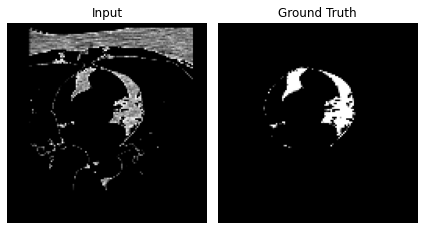
\includegraphics[width=0.49\columnwidth]{images/4/eat_example}} \\
	\caption{Example input images and ground-truth labels for each dataset used in our experiments. \cite{bencevicTrainingPolarImage2021}}
	\label{fig:datasets}
	\end{figure*}

\textbf{Polyp dataset:} The CVC-ClinicDB dataset
\cite{bernalWMDOVAMapsAccurate2015} contains 612 RGB 
colonoscopy images with the resolution $288 \times 384$ 
with labeled polyps from MICCAI 2015. We normalize each image to a range of $[-0.5, 0.5]$. 
We use the original image resolution to train all networks except the 
centerpoint network. As is used in \cite{jhaDoubleUNetDeepConvolutional2020}, 
we use an 80\%, 10\% and 10\% 
split for training, validation, and testing datasets, respectively. An example of the dataset is shown in \figref{fig:datasets}(a).

\textbf{Liver dataset:} The second dataset we use is the LiTS dataset \cite{bilicLiverTumorSegmentation2019} from the Liver Tumor Segmentation Challenge from MICCAI 2017. The dataset contains 131 CT scans of patients with hepatocellular carcinoma, with the liver as well as tumor lesions labeled by experts. In our experiments, we disregard the lesion segmentation labels and treat the dataset as a binary liver segmentation problem. In addition, we removed all slices that did not contain a ground-truth liver segmentation label, resulting in a dataset of roughly 15,000 slices. Each axial slice is thresholded to a Hounsfield scale range of $[0, 200]$ HU that contains the liver. Next, the slices are normalized to a $[0, 1]$ range and zero-centered by subtracting the global intensity of all training slices (0.1). We then proceed to train the networks on each axial slice separately. We use 101 scans for training, 15 scans for validation, and the remaining 15 scans for testing. Example liver segmentation images are shown in \figref{fig:datasets}(c).

\textbf{Lesion dataset:} The third dataset we use is the ISIC 2018 Lesion Boundary Segmentation dataset 
\cite{codellaSkinLesionAnalysis2018, tschandlHAM10000DatasetLarge2018} which contains 2,694 dermatoscopy 
images of skin lesions with expert labels of the lesions from various anatomic sites and several different 
institutions. We resize each image to a 
resolution of $384 \times 512$ and use a training, validation, and test split of 80\%, 10\%, and 10\%, 
respectively. This is consistent with \cite{jhaDoubleUNetDeepConvolutional2020}. Additionally, we normalize 
each image to a range of $[-0.5, 0.5]$. An example of a lesion 
input image and its corresponding label is shown in \figref{fig:datasets}(b).

\textbf{EAT dataset:} Finally, we also train on a dataset of labeled EAT regions from 20 patients' cardiac CT scans from 
the Cardiac Fat Database \cite{rodriguesNovelApproachAutomated2016}. The dataset has three classes labeled: 
the pericardium, EAT, and pericardial adipose tissue. We disregard all original labels except EAT and treat the dataset as a binary EAT segmentation dataset. The dataset is 
first split into training (10 patients), validation (5 patients), and test (5 patients) datasets. In the 
original dataset, 
each slice is thresholded to the adipose tissue range of $[-200, -30]$ HU and registered so that anatomical 
structures have the same locations. In addition to these original pre-processing steps, we normalize each 
slice to a $[0, 1]$ range and zero-center 
the dataset by subtracting a global mean intensity of the training set (0.1). We then train on 
each CT slice separately. An input image of the EAT dataset and its corresponding label is shown in 
\figref{fig:datasets}(d).

    \subsubsection{Implementation details}

We use the OpenCV linear polar transformation implementation.
Each model is implemented and trained using PyTorch 1.7.1 on an NVIDIA GeForce RTX 3080 GPU. For all 
networks, we use the Adam optimizer with a learning rate of $10^{-3}$. A batch size of 8 was used for all 
networks except the center-point model, where a batch size of 6 was used for the lesion and liver datasets 
and 8 for all remaining datasets. We trained all models up to a maximum of 200 epochs and used checkpoints 
after each epoch to store the model with the best validation loss. We modify the Dice coefficient to act as a loss function as follows:
  \begin{equation}
    \textit{DSC}_{loss} = 1 - \frac {2\lvert X\cap Y\rvert + \lambda}{\lvert X\rvert + \lvert Y\rvert + \lambda},
    \label{eq:dice-loss}
  \end{equation}
where $X$ and $Y$ are the input and predicted images, respectively, and $\lambda$ is a smoothing parameter set to 1 in our experiments used to avoid dividing by zero.
This loss function is used to train all models except the center-point model.

The centerpoint model outputs eight heatmaps \cite{newellStackedHourglassNetworks2016}. 
We use a loss function that is the mean of the mean squared errors between each of the heatmaps and the ground truth heatmap.
The code used for all experiments is available at \url{github.com/marinbenc/medical-polar-training}.

  \subsection{Results and Discussion}

% ---------- RESULT  TABLES ---------- %

\begin{table}[t!]
\centering
\def\arraystretch{1.2}
\begin{tabularx}{\textwidth}{X X c c c c} 
 \\ [-2ex]

 \multicolumn{6}{c}{\textbf{Polyp Segmentation}}\\[1ex]
 \hline
 Architecture & Method & DSC & mIoU & Prec. & Rec. \\ 
 \hline \\ [-1.5ex]
 
 \multirow{4}{7em}{{U-Net}}
& Cartesian & 0.8315 & 0.7604 & 0.8513 & 0.8334 \\
& GT centers & 0.9484 & 0.9141 & 0.9563 & 0.9442 \\
& Cart. centers & 0.8973 & 0.8571 & 0.8996 & 0.8998 \\
& Model centers & 0.9374 & 0.8977 & 0.9488 & 0.9368 \\ [1ex]
\hline \\ [-1.5ex]

 \multirow{4}{7em}{{Res-U-Net++}}
& Cartesian & 0.8356 & 0.7636 & 0.9004 & 0.8256 \\
& GT centers & 0.9557 & 0.9260 & 0.9583 & 0.9554 \\
& Cart. centers & 0.9063 & 0.8685 & 0.9243 & 0.9027 \\
& Model centers & 0.9332 & 0.8924 & 0.9477 & 0.9321 \\ [1ex]
\hline \\ [-1.5ex]

 \multirow{4}{7em}{{DeepLabV3+}}
& Cartesian & 0.8706 & 0.8013 & 0.8857 & 0.8876 \\
& GT centers & 0.9593 & 0.9296 & 0.9576 & 0.9682 \\
& Cart. centers & 0.9212 & 0.8823 & 0.9179 & 0.9397 \\
& Model centers & 0.9338 & 0.8967 & 0.9436 & 0.9347 \\ [1ex]
\hline \\ [-1.5ex]

\multicolumn{6}{c}{\textbf{Lesion Segmentation}}\\[1ex]
 \hline
  & Method & DSC & mIoU & Prec. & Rec. \\ 
 \hline \\ [-1.5ex]
 
 \multirow{4}{7em}{{U-Net}}
& Cartesian & 0.8256 & 0.7393 & 0.8407 & 0.8712 \\
& GT centers & 0.9320 & 0.8824 & 0.9261 & 0.9541 \\
& Cart. centers & 0.8836 & 0.8317 & 0.8746 & 0.9492 \\
& Model centers & 0.9224 & 0.8699 & 0.9165 & 0.9494 \\ [1ex]
\hline \\ [-1.5ex]

 \multirow{4}{7em}{{Res-U-Net++}}
& Cartesian & 0.8664 & 0.7925 & 0.8728 & 0.9122 \\
& GT centers & 0.9439 & 0.9014 & 0.9418 & 0.9584 \\
& Cart. centers & 0.9125 & 0.8653 & 0.9075 & 0.9540 \\
& Model centers & 0.9253 & 0.8743 & 0.9253 & 0.9464 \\ [1ex]
\hline \\ [-1.5ex]

 \multirow{4}{7em}{{DeepLabV3+}}
& Cartesian & 0.8717 & 0.7984 & 0.8807 & 0.9068 \\
& GT centers & 0.9459 & 0.9059 & 0.9418 & 0.9632 \\
& Cart. centers & 0.9162 & 0.8686 & 0.9097 & 0.9536 \\
& Model centers & 0.9235 & 0.8721 & 0.9125 & 0.9570 \\ [1ex]
\end{tabularx}
\caption{Results of our proposed approaches for different tasks 
for three different neural network architectures. The Cartesian network is the network trained on Cartesian images. ``GT centers'' refers to obtaining a polar origin from the ground-truth labels and segmentation using the polar network.``Cartesian centers'' refers to predicting the polar origins from the Cartesian network and then performing segmentation using the polar network. ``Model centers'' refers to using the centerpoint predictor to obtain polar origins. (Continued on the next page.)}
\label{table:results}
\end{table}

\begin{table}[t!]
\ContinuedFloat
\centering
\def\arraystretch{1.2}
\begin{tabularx}{\textwidth}{X X c c c c} 
\\ [-2ex]
\multicolumn{6}{c}{\textbf{Liver Segmentation}}\\[1ex]
 \hline
 Segm. net. & Method & DSC & mIoU & Prec. & Rec. \\ 
 \hline \\ [-1.5ex]
 \multirow{4}{7em}{{U-Net}}
& Cartesian & 0.8976 & 0.8505 & 0.8997 & 0.9201 \\
& GT centers & 0.9553 & 0.9227 & 0.9595 & 0.9569 \\
& Cart. centers & 0.9302 & 0.8985 & 0.9279 & 0.9429 \\
& Model centers & 0.9125 & 0.8828 & 0.9108 & 0.9219 \\ [1ex]
\hline \\ [-1.5ex]

 \multirow{4}{7em}{{Res-U-Net++}}
& Cartesian & 0.8908 & 0.8463 & 0.8936 & 0.9085 \\
& GT centers & 0.9548 & 0.9215 & 0.9492 & 0.9661 \\
& Cart. centers & 0.9219 & 0.8898 & 0.9119 & 0.9428 \\
& Model centers & 0.9109 & 0.8795 & 0.9009 & 0.9306 \\ [1ex]
\hline \\ [-1.5ex]

 \multirow{4}{7em}{{DeepLabV3+}}
& Cartesian & 0.8868 & 0.8341 & 0.8995 & 0.8959 \\
& GT centers & 0.9518 & 0.9171 & 0.9547 & 0.9550 \\
& Cart. centers & 0.9253 & 0.8932 & 0.9244 & 0.9361 \\
& Model centers & 0.9092 & 0.8783 & 0.9075 & 0.9199 \\ [1ex]
\hline \\ [-1.5ex]

\multicolumn{6}{c}{\textbf{Epicardial Fat Segmentation}}\\[1ex]
 \hline
 Segm. net. & Method & DSC & mIoU & Prec. & Rec. \\ 
 \hline \\ [-1.5ex]
 \multirow{4}{7em}{{U-Net}}
& Cartesian & 0.7544 & 0.5812 & 0.7190 & 0.6949 \\
& GT centers & 0.8088 & 0.6607 & 0.7986 & 0.7675 \\
& Cart. centers & 0.7835 & 0.6227 & 0.7455 & 0.7208 \\
& Model centers & 0.7840 & 0.6252 & 0.7451 & 0.7302 \\ [1ex]
\hline \\ [-1.5ex]

 \multirow{4}{7em}{{Res-U-Net++}}
& Cartesian & 0.3410 & 0.1743 & 0.2700 & 0.3294 \\
& GT centers & 0.8030 & 0.6827 & 0.7939 & 0.8043 \\
& Cart. centers & 0.5466 & 0.3980 & 0.5286 & 0.5066 \\
& Model centers & 0.7740 & 0.6140 & 0.7156 & 0.7453 \\ [1ex]
\hline \\ [-1.5ex]

 \multirow{4}{7em}{{DeepLabV3+}}
& Cartesian & 0.6380 & 0.4246 & 0.5665 & 0.5940 \\
& GT centers & 0.6952 & 0.5123 & 0.6519 & 0.6779 \\
& Cart. centers & 0.6696 & 0.4716 & 0.5988 & 0.6454 \\
& Model centers & 0.6720 & 0.4779 & 0.6070 & 0.6488 \\ [1ex]
\end{tabularx}
\caption{Results of our proposed approaches (continued).}
\label{table:results}
\end{table}

We evaluate segmentation performance along with four key metrics: the Dice coefficient (DSC), the median intersection-over-union score (mIoU), precision, and accuracy. Precision and accuracy are both calculated pixel-wise. The results of training the different approaches presented in \ref{experiments} are shown in \tabref{table:results} for polyp, lesion, liver, and EAT segmentation. In all cases, training on polar coordinates improves the segmentation in all metrics when compared to training the same model on Cartesian coordinates. As is to be expected, testing the polar network on images transformed using the ground truth polar origins produces the best results in terms of DSC. A close second predicts the polar origin from the center-point predictor. Predicting polar origins from the Cartesian model leads to less accurate polar origins, and the results are worse in terms of DSC, however, they are still better than using only the Cartesian model.

We also compare our methods to other state-of-the-art methods that use the same datasets, shown in \tabref{table:comparison}. We achieve state-of-the-art results for the polyp and liver datasets. Additionally, we achieve state-of-the-art liver segmentation when compared to other per-slice methods, and nearly state-of-the-art results when compared to 3D-based methods. For EAT segmentation, our approach outperforms standard medical image segmentation networks but does not achieve state-of-the-art performance due to segmenting EAT directly and not first segmenting the pericardium.

\begin{table}[t]
\centering
\def\arraystretch{1.2}
\begin{tabularx}{\textwidth}{X X c c c c} 
 \textbf{Dataset} & \textbf{Method} & \textbf{DSC} & \textbf{mIoU} & \textbf{Prec.} & \textbf{Rec.} \\ 
 \hline \\ [-1.5ex]
 
 \multirow{3}{1em}{{Polyp}}
& PraNet \cite{fanPraNetParallelReverse2020} & 0.8990 & 0.8490 & - & - \\
& FANet \cite{tomarFANetFeedbackAttention2021a} & - & 0.8937 & 0.9401 & 0.9339 \\
& Our method & \textbf{0.9374} & \textbf{0.8977} & \textbf{0.9488} &  \textbf{0.9368} \\ [1ex]
\hline \\ [-1.5ex]

 \multirow{3}{1em}{{Lesion}}
& DeepLabV3+ \cite{chenEncoderDecoderAtrousSeparable2018} & 0.8717 & 0.7984 & 0.8807 & 0.9068 \\
& DoubleU-Net \cite{jhaDoubleUNetDeepConvolutional2020} & 0.8962 & 0.8212 & \textbf{0.9459} & 0.8780 \\
& Our method & \textbf{0.9253} & \textbf{0.8743} & 0.9253 &  \textbf{0.9464} \\ [1ex]
\hline \\ [-1.5ex]

 \multirow{3}{1em}{{Liver}}
& U-Net \cite{ronnebergerUNetConvolutionalNetworks2015} & 0.8976 & 0.8505 & 0.8997 & 0.9201 \\
& KiU-Net 3D \cite{valanarasuKiUNetOvercompleteConvolutional2020a} & \textbf{0.9423} & 0.8946 & - & - \\
& Our method & 0.9302 & \textbf{0.8985} & 0.9279 & 0.9429 \\ [1ex]
\hline \\ [-1.5ex]

 \multirow{3}{1em}{{EAT}}
& U-Net. \cite{ronnebergerUNetConvolutionalNetworks2015} & 0.7544 & 0.5812 & 0.7190 & 0.6949 \\
& Zhang et al. \cite{zhangAutomaticEpicardialFat2020a} & \textbf{0.9119} & \textbf{0.8425} & - & - \\
& Our method & 0.7840 & 0.6252 & 0.7451 &  0.7302 \\ [1ex]
\end{tabularx}
\caption{A comparison between our method (approach with best results) and the state of the art on the same datasets.}
\label{table:comparison}
\end{table}

% ---------- END RESULT TABLES ---------- %

A training graph for a polar and Cartesian U-Net-based network is shown in \figref{fig:training}. Additionally, we evaluate the accuracy of the different ways of obtaining the polar origin. This accuracy is compared with segmentation performance in \figref{fig:centers-vs-performance}.

	\begin{figure}[b!]
		\centering
		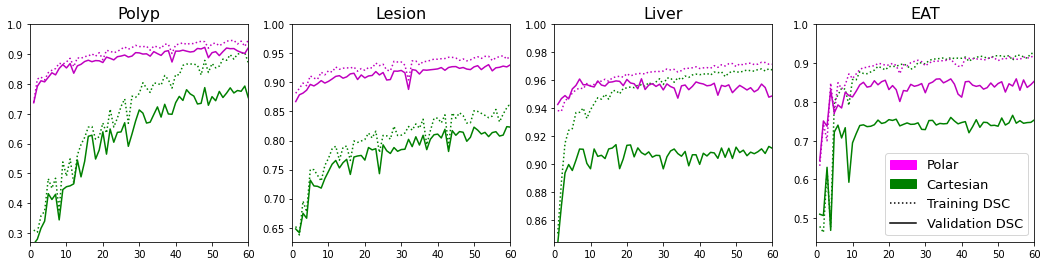
\includegraphics[width=\linewidth]{images/4/training-graphs}
		\caption{The training and validation Dice coefficient (DSC) of the polar and Cartesian U-Net models during training. \cite{bencevicTrainingPolarImage2021}}
		\label{fig:training}
	\end{figure}
		
We also train several models with both polar and Cartesian coordinates on subsets of the training dataset. Namely, we trained models on 25\%, 50\%, 75\%, and 100\% of the lesion training dataset for 50 epochs. The results of this training are shown in \figref{fig:dataset-vs-dsc}. The polar network is much more data efficient and achieves better results than the cartesian network even with only 25\% of the data.

	\begin{figure}[t!]
		\centering
		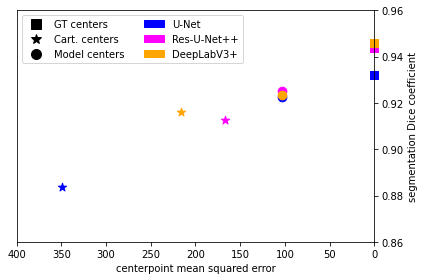
\includegraphics[width=0.65\linewidth]{images/4/mse-vs-dice}
		\caption{The relationship between mean squared errors of the centers used for the polar transformation and segmentation performance of the polar network on the lesion dataset. The mean squared errors are calculated compared to the ground-truth centers. \cite{bencevicTrainingPolarImage2021}}
		\label{fig:centers-vs-performance}
	\end{figure}
	
	\clearpage
	
			\begin{figure}[t!]
		\centering
		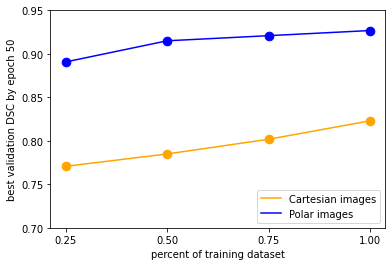
\includegraphics[width=0.65\linewidth]{images/4/dsc-vs-dataset-percent}
		\caption{The best Dice coefficient by epoch 50 for models trained on subsets of the lesion training dataset. \cite{bencevicTrainingPolarImage2021}}
		\label{fig:dataset-vs-dsc}
	\end{figure}
	
		\subsubsection{Discussion}
	
We obtain state-of-the-art results for polyp and lesion segmentation by training common biomedical image segmentation models. In the liver dataset, we achieve state-of-the-art results when compared to other 2D methods, but 3D methods 
achieve the same or slightly better results \cite{valanarasuKiUNetOvercompleteConvolutional2020a}. 
The liver dataset is 
by far the largest dataset we evaluated. As such, improvements gained from 
encoding localization information and reducing dimensionality might not be as large as in smaller 
datasets, since the network has enough data to learn these complex structures.
The EAT dataset is one where the task is not to find a single object, but instead, to segment multiple smaller 
pockets of tissue around the heart. This task is more challenging for common models like U-Net and 
requires a more complex approach \cite{zhangAutomaticEpicardialFat2020a}. It is possible that combining 
these existing approaches, namely segmenting the pericardium first, with training on polar coordinates 
would lead to an improvement in the state of the art.

	\begin{figure*}[b!]
	\subfloat[Polyp predictions]{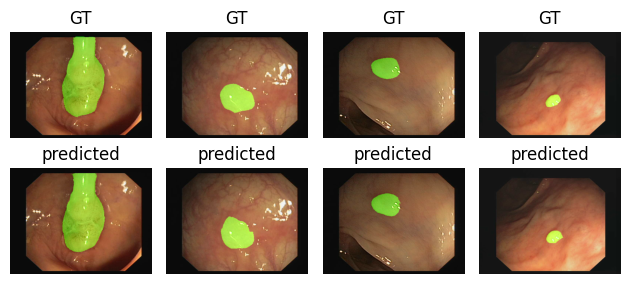
\includegraphics[width=0.49\columnwidth]{images/4/centerpoint_model_output_polyp}}
	\hfill
	\subfloat[Lesion predictions]{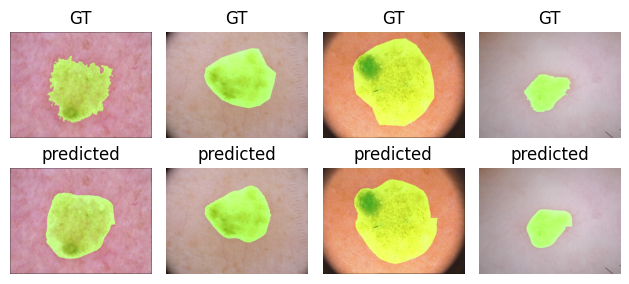
\includegraphics[width=0.49\columnwidth]{images/4/centerpoint_model_output_lesion}} \\
	\subfloat[Liver predictions]{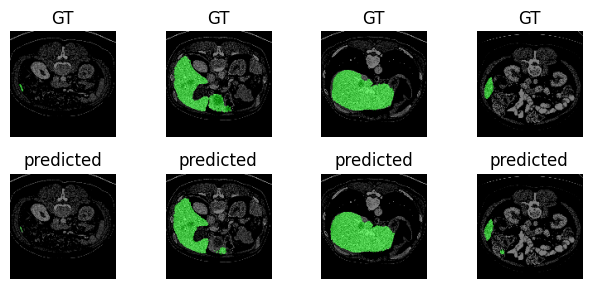
\includegraphics[width=0.49\columnwidth]{images/4/centerpoint_model_output_liver}}
	\hfill
	\subfloat[EAT predictions]{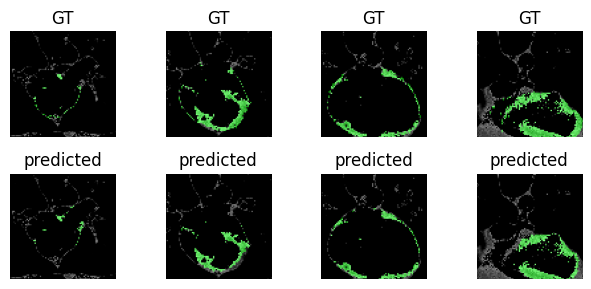
\includegraphics[width=0.49\columnwidth]{images/4/centerpoint_model_output_eat}} \\
	\caption{A random sampling of inverse polar transformed predictions from the polar network with the polar origins predicted from the centerpoint predictor for various datasets. The prediction is shown in green and overlaid on top of the original input image. EAT predictions (d) are cropped and zoomed to better show the predictions. \cite{bencevicTrainingPolarImage2021}}
	\label{fig:predictions}
	\end{figure*}

We also show that training on polar images leads to a significant improvement in segmentation performance 
when compared to training on Cartesian images for the same network architecture. Additionally, as shown in \figref{fig:training}, the polar 
network portions of our approach converge in much fewer epochs than the Cartesian networks. This is in part due to the location information being encoded in the image 
itself via the polar origin, and in part due to a possible data dimensionality reduction, allowing the 
network to more easily optimize the loss function. The polar networks are also more robust to low dataset 
sample size. This is especially important in biomedical image segmentation where the availability of large 
labeled datasets is often very limited.

Predicting the center point from the Cartesian model, while still an improvement over the plain 
Cartesian network leads to slightly lower DSC results than those obtained by the center point predictor model. 
We conclude that segmentation is highly dependent on choosing the correct polar origin. This 
dependency is somewhat loosened by adding polar origin augmentation when training the polar 
network.

	\begin{table}[t]
\centering
\def\arraystretch{1.2}
\begin{tabularx}{\linewidth}{X c c}
 Method & DSC & Difference \\ 
 \hline \\ [-2ex]
Cartesian & 0.8315 & - \\
Polar (Cartesian origins) & 0.8918  & +0.0603 \\
Polar (Centerpoint predictor) & 0.9094 & +0.0176  \\
 + centerpoint augmentation & 0.9288 & +0.0194 \\
 + polar network training augmentation & 0.9374 & +0.0086 \\ [1ex]
\end{tabularx}
\caption{Ablation study of our approach for the polyp dataset.}
\label{table:ablation}
\end{table}

\figref{fig:predictions} shows a random sampling of predictions from the polar network using the center point predictor for polar origins. Qualitatively, we conclude that the network segmentation achieves a high overlap with the target object. The network successfully segments both small and elliptical as well as large and unevenly shaped polyps. On the lesion images, the network predicts a smooth border when sometimes the actual border of the lesion is rough, as shown in the left-most example on \figref{fig:predictions}(b), however, the network still does a good job of delineating a lesion border even when the color of the lesion is very similar to the surrounding skin. The network successfully predicts a liver border both when the liver is very large and very small on the image, showing good scale invariance, but sometimes under segments the liver when multiple connected components are needed. On the EAT dataset, the network successfully learns to segment EAT despite its highly discontinuous and sparse distribution. However, the network sometimes under segments EAT.

Finally, we also perform an ablation study shown in \tabref{table:ablation}. Training on the polar coordinates with the polar origins predicted from the cartesian network yields the largest performance improvement. Predicting the polar origin from the center point predictor as well as adding center point augmentation to the predictor play a roughly equally important role in the performance. Lastly, a small performance improvement is further achieved by using data augmentation when training the polar network.

The center points could also be obtained by a more basic segmentation approach 
like thresholding or other traditional image processing methods, leading to a possible reduction in the 
number of required neural network parameters to achieve good segmentation. Furthermore, in our experiments,
we found that the segmentation is dependent on choosing the correct standard deviation of the generated 
heatmaps for training the center point predictor. An improvement to our method could be made by developing
a method to automatically estimate the standard deviation from the training or validation data without needing
to first train the center point predictor.

In conclusion, the polar transform demonstrates significant potential in simplifying the segmentation of elliptical objects, thus reducing the complexity of the neural network model required. However, a key limitation of this approach is that only one elliptical object can be segmented. The next section will introduce further advancements to this method, allowing the segmentation of multiple objects on the image.

\section{Supporting Multiple Transformations of an Image}

In this chapter, we've explored an approach where each image undergoes a single transformation before being processed by the segmentation network. We will now extend this model-driven preprocessing approach to accommodate multiple transformations of the same input image. This modification is particularly useful in scenarios where an image contains several objects, each with its distinct decision boundary. By applying a separate polar transformation for each object center, we can generate multiple segmentation maps for a single image. These maps can then be combined to create a unified segmentation result. The process involves the following steps:

\begin{enumerate}
	\item Our transformation predictor network will be enhanced to predict a set of transformation parameters \(\{\phi_1, \phi_2, \cdots, \phi_n\}\), where \(n\) varies based on the image and represents the number of transformations.
	\item For each transformation parameter in $\phi_i$ we will produce a corresponding set of transformed images $\{I'_i\}$, $I'_i = \mathcal{T}_{\phi_i}(I)$.
	\item Each transformed image $I'_i$ will be segmented using the segmentation network, producing a series of segmentation maps \(\{M_i\}\), where \(M_i = F_{seg}(I'_i)\).
	\item Finally, all of the segmentations will be fused using an aggregation function $f_{agg}$, resulting in a final segmentation map $M = f_{agg}(\{M_i\})$.
\end{enumerate}

To exemplify this, we will present a case of using the polar transformation as we did earlier, only this time we will be segmenting images with multiple connected components (objects) in their segmentation maps. Therefore, we will use multiple polar transformations for each image, one for each connected component. The transformation parameter predictor will be modified to predict the centroid of each connected component, instead of just a single centroid. Each centroid will be used to transform and segment the image. For the aggregation function, we will choose a weighted sum and a hysteresis thresholding function $th$ with thresholds $t_1$ and $t_2$:
\begin{equation}
	f_{agg}(\{M_i\}) = th(\sum_{i = 1}^n M_i W_i; t_1, t_2),
\end{equation}
each weight \(W_i\) functions as an image matching the dimensions of \(M_i\), where the pixels correspond to the relative importance of that pixel in the corresponding segmentation map. For instance, in the case of the polar transform, the value assigned to each element in \(W_i\) depends on its relation to the connected component associated with the polar origin for the corresponding segmentation mask \(M_i\). Specifically, elements that belong to the same connected component as the polar origin used for the \(i\)-th segmentation are assigned a value of 2. Elements outside this connected component are assigned a value of 1. With this weighing strategy, regions belonging to the connected component that is most beneficially transformed are more heavily weighted than other pixels.

		\begin{figure}[b!]
		\centering
		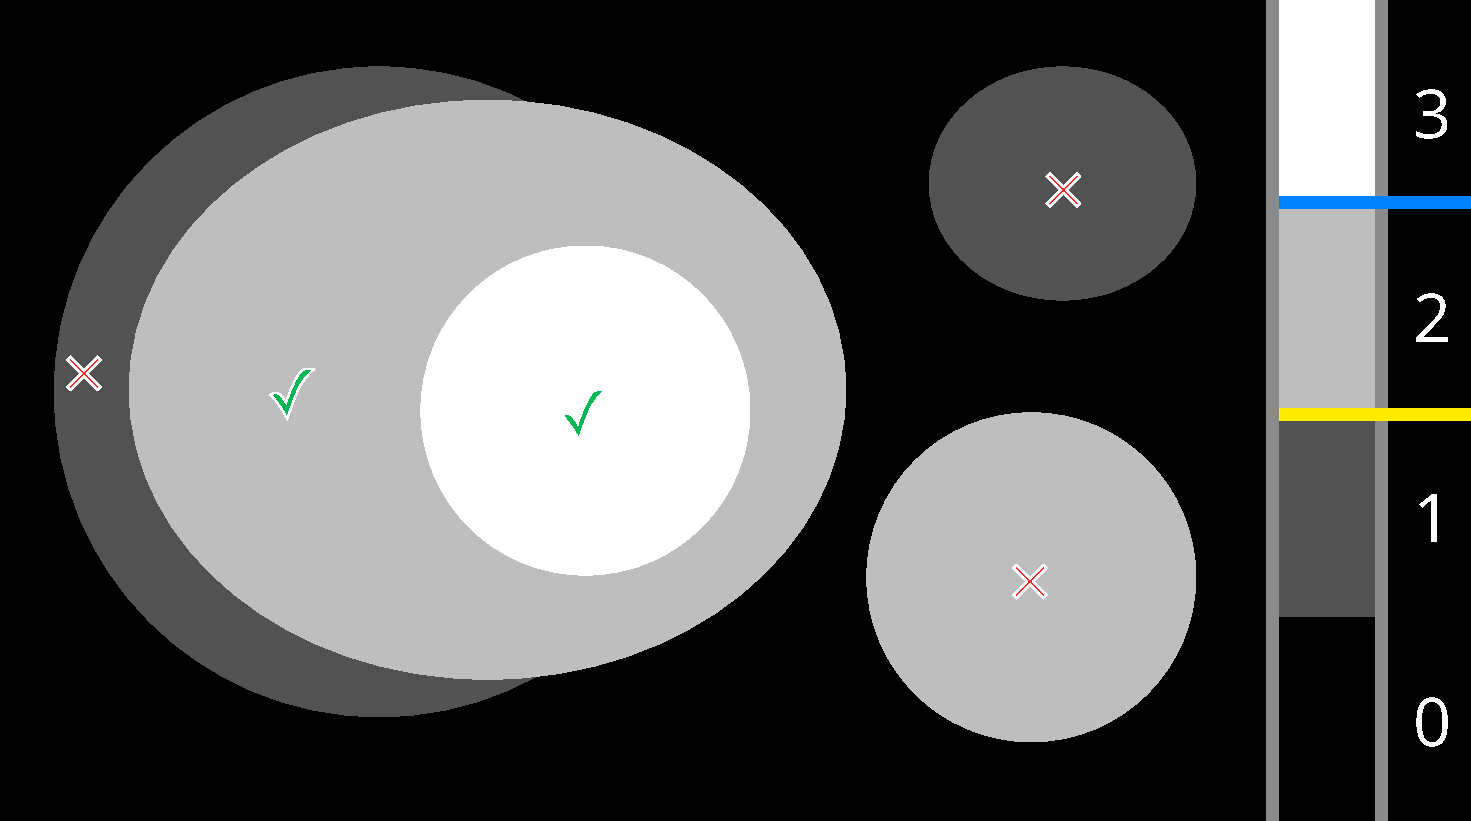
\includegraphics[width=0.5\linewidth]{images/4/hysteresis-ccs}
		\caption{A visual explanation of hysteresis thresholding. Kept regions are marked with green checkmarks, while deleted regions are marked with red crosses. The pixel intensity scale is shown on the right, where $t_1$ is marked in yellow and $t_2$ is marked in blue.}
		\label{fig:hysteresis-ccs}
	\end{figure}

The hysteresis thresholding function \(th\), defined by two thresholds \(t_1\) and \(t_2\), operates in two stages. Initially, it eliminates all pixels with intensity levels below \(t_1\). First, it removes all pixels with an intensity lower than $t_1$. Next, in the remaining pixels of the image, for each connected component, if any of the component's pixel intensities are higher than $t_2$, the whole connected component is preserved, otherwise the connected component is removed, as illustrated in \figref{fig:hysteresis-ccs}.
	
The approach of model-driven preprocessing using multiple transformations has several advantages. First, each object can benefit from the reduction in segmentation complexity. For example, in the case of the polar transform, one object is always the bottom part of the polar transformed image to be segmented, so the network does not need to learn to first localize the object. Secondly, a consequence of this approach is that images with multiple connected components are over-sampled during training. This is beneficial since these images are usually under-represented (when compared to images with fewer connected components) and harder to segment (since they require segmenting multiple objects).
	
What follows is an empirical study of this approach for aorta segmentation, which is a modification of the one presented in \ref{polar-paper} to allow support for multiple transformations of the input image, one for each object in the image.

\section{Model-Driven Preprocessing using Multiple Transformations for Aorta Segmentation}

The aorta is the largest artery of the human body and supplies oxygenated blood from the heart to all parts of the body. It is one of the most clinically significant structures to analyze for cardiovascular disease diagnosis and prevention. Several conditions could occur on the aorta which can be detected using 3D medical imaging, including aneurysms, dissections, stenoses, coarctations, or traumas. All of these conditions can be dangerous and require careful screening, following, and potentially surgical treatment, while a failure or delay in the diagnosis of these conditions could be fatal. Therefore, developing a fully automated method to efficiently and accurately segment the aorta could be beneficial for earlier detection of these conditions. By producing a 3D model of the aorta from CT or MRI scans, a computer algorithm could perform automatic measurements to screen and detect aortic aneurysms, dissections, and other conditions that are commonly diagnosed by imaging the aorta.

Several methods based on deep learning were proposed for segmenting the aorta from CT images. \citet{fantazzini3DAutomaticSegmentation2020} use a cascade of U-Net-based networks. They first perform a rough segmentation on axial slices to extract a region of interest. They then use separate networks to segment axial, sagittal, and coronal slices of the region of interest. Several other papers have used 3D U-Net-based architectures for this task \cite{yuThreeDimensionalDeepConvolutional2021, chenMultistageLearningSegmentation2021}.

\subsection{Methodology}

The approach presented in this section is an extension of the approach presented in \ref{polar-paper}. We obtain the center points of the objects in the image using a rough segmentation from a U-Net-based network, instead of using a center point predictor as is described in \ref{polar-paper}. A summary of the approach is shown in \figref{fig:summary}.

\begin{figure}[t!]
\centering
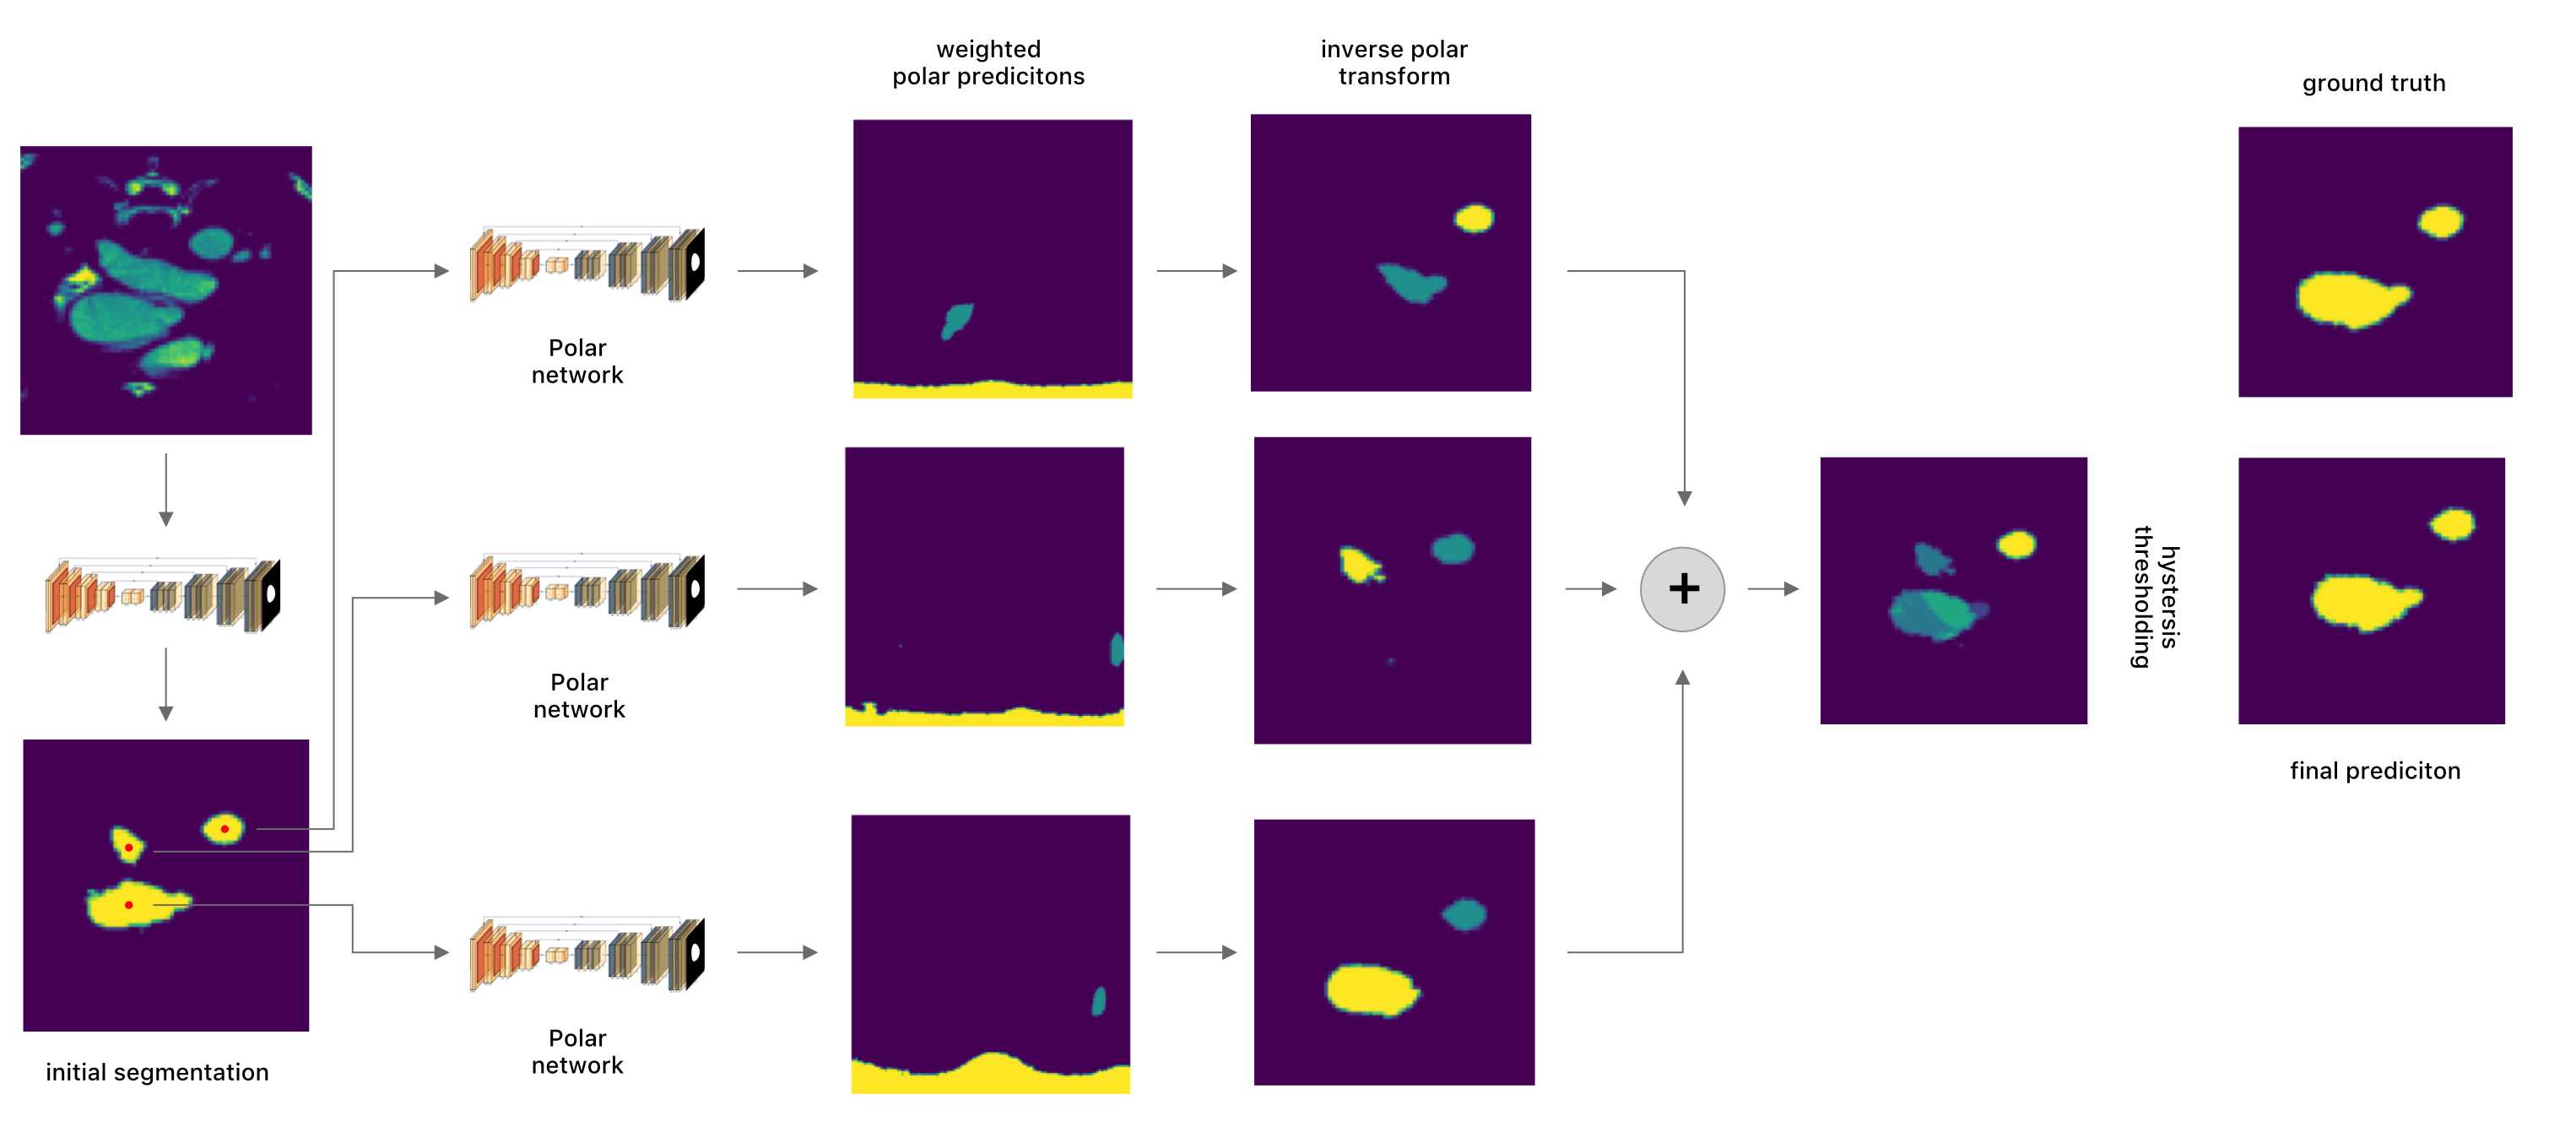
\includegraphics[width=\textwidth]{images/4/summary}
\caption{A summary of our approach. An input image is first segmented using a U-Net network. For each connected component in the segmentation, the input image is transformed to polar coordinates using the centroid of the connected component as the origin. These images are then fed into a U-Net trained on polar images, and the predictions for each object are fused, hysteresis thresholded, and transformed back to cartesian coordinates. Note how one of the false positive connected components in the initial segmentation was removed during hysteresis thresholding since the component was only predicted in one of the three polar predictions. \cite{bencevicUsingPolarTransform2022a}}
\label{fig:summary}
\end{figure}

As described earlier in this section, we perform several key modifications to allow the network to segment multiple objects on an image. During the training of the polar network, we construct a dataset that contains one polar transformation per connected component in the ground truth segmentation label. The origins of these polar transformations are the centroid of each corresponding connected component.

We also employ prediction fusion during inference. First, a 2D U-Net-based network is used to obtain an initial rough segmentation. A separate polar transformation for each connected component in the rough segmentation is constructed using the centroid of each component as the origin. The polar network predicts a segmentation map for each transform, resulting in a number of predictions equal to the number of connected components. In the predicted image, a weight of 2 is assigned to the connected component which contains the origin for that prediction, and a weight of 1 to all other connected components. We then sum all of the weighted images together. As shown earlier in this chapter, the polar network generally performs best on objects which contain the polar origin, and worse at predicting other objects on the image. Therefore, we assign a larger weight to that component as a proxy for a confidence measure. We then sum all of the weighted predictions together and normalize the prediction to a 0-1 range. This leads to a segmentation map where each non-zero pixel represents the confidence that the pixel belongs to the aorta class. To obtain the final segmentation, we use hysteresis thresholding where the bottom threshold is 0, and the top threshold is 0.4, empirically determined according to the best Dice coefficient on the validation dataset. An example of thresholding a prediction is shown in \figref{fig:thresh}.

\begin{figure}[t!]
\centering
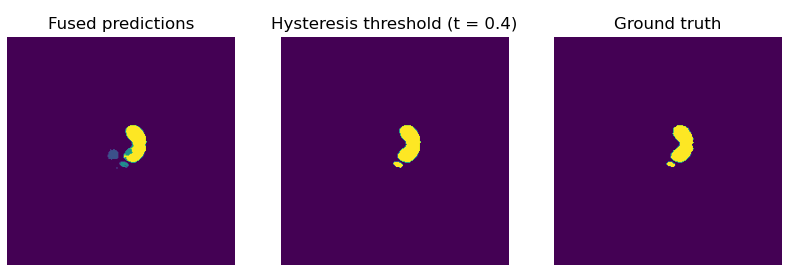
\includegraphics[width=0.8\columnwidth]{images/4/hyst}
\caption{Hystersis-thresholded segmentation output. For each polar prediction, the component that contains the origin of the transform gets a weight of 2 assigned, while all other components get a weight of 1. This left-most image is the result of summing the predictions of 3 polar transformations of the original image (one for each connected component), converted to cartesian coordinates. Note how the thresholding removes the false positive object on the left of the image while keeping the true positive objects intact. \cite{bencevicUsingPolarTransform2022a}}
\label{fig:thresh}
\end{figure}

\subsubsection{Data Description and Preprocessing}

We used a publicly available dataset of CT scans with corresponding aorta labels \cite{radlAVTMulticenterAortic2022} including the ascending aorta, the aortic arch as well as the descending and abdominal aorta. While the original dataset contains scans from three different centers, in our experiments, we only use the data from Dongyang Hospital. In total, we use 18 CT scans, each containing 122-251 slices, with a slice thickness of 2 or 3 mm.

Each CT slice is windowed to a range of 200 to 500 HU to remove information from irrelevant tissues, then normalized to a range of -0.5 to 0.5, and zero centered using the global mean value across all slices in the validation set. The slices were each resized from $512 \times 666$ to $256 \times 256$ pixels. We use augmentation during training for both the cartesian and the polar network. The augmentations we use include a $50\%$ chance of a random combination of affine transforms including a shift of up to $6.25\%$, a scale of up to $10\%$ and a rotation of up to $15^{\circ}$; as well as a $30\%$ chance of a horizontal flip.

All of our models were implemented using PyTorch 3.9 using an NVIDIA GeForce RTX 3080 GPU. We use the U-Net \cite{ronnebergerUNetConvolutionalNetworks2015d} architecture for both the cartesian and the polar network. For training, we use a batch size of 8 and the Adam optimizer with a learning rate of $0.001$. All models were trained for 60 epochs with checkpointing where the model with the best validation Dice coefficient was selected. We use the Dice loss function as described in the previous section of this chapter. All of the code, as well as the trained networks, can be found at \href{https://github.com/marinbenc/medical-polar-training}{github.com/marinbenc/medical-polar-training}.

\subsection{Results and Discussion}

\begin{figure}[b!]
\centering
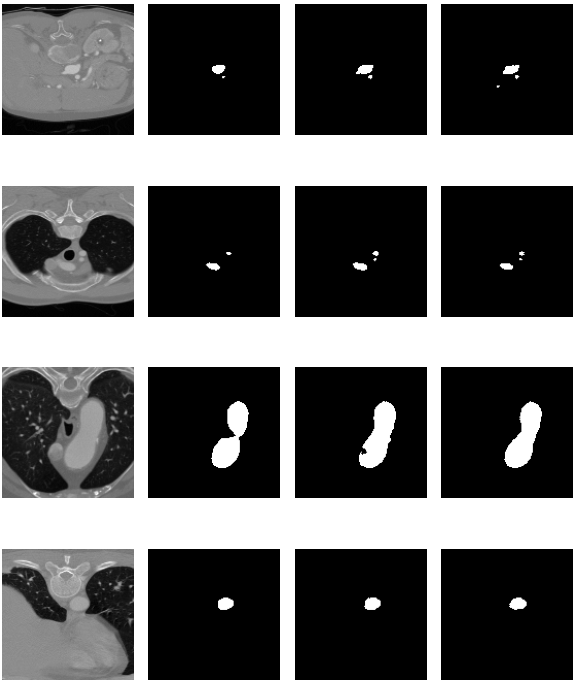
\includegraphics[width=\columnwidth]{images/4/examples_3}
\caption{Random examples of predictions. Columns from left to right show: the input image, the initial prediction from the non-polar network, the final fused polar prediction, and the ground truth segmentation label. \cite{bencevicUsingPolarTransform2022a}}
\label{fig:examples}
\end{figure}

\begin{table}[b!]
\def\arraystretch{1.2}
\centering
\begin{tabularx}{\linewidth}{X c c c c} 
 \textbf{Method} & \textbf{DSC} & \textbf{mIoU} & \textbf{Prec.} & \textbf{Rec.} \\ 
 \hline
U-Net (non-polar) & $0.886 \pm 0.049$ & $0.825 \pm 0.052$ & $0.901 \pm 0.074$ & $0.893 \pm 0.039$ \\
Polar + GT centers & $0.937 \pm 0.053$ & $0.895 \pm 0.055$ & $0.944 \pm 0.064$ & $0.937 \pm 0.040$ \\
Polar + NP centers* & $0.932 \pm 0.027$ & $0.895 \pm 0.033$ & $0.915 \pm 0.040$ & $0.973 \pm 0.018$ \\
\end{tabularx}
\caption{A summary of the mean segmentation results of our experiments. \textit{Non-polar} are the results of the U-Net trained using cartesian images. \textit{Polar + GT centers} are the results of the U-Net trained on polar images, using ground-truth connected component centers during inference, as an example of the best case possible results. \textit{Polar + NP centers} are the results when running inference on the polar model using center points obtained from the non-polar model predictions. *Our proposed method.}
\label{table:results}
\end{table}

To perform evaluation, we use 3-fold cross-validation on the 18 scans. For each fold, we train a polar and non-polar model using the slices of 12 CT scans and run inference on the slices of the remaining 6 scans. All results presented in this section are averaged across each CT scan and then across the three folds.

A summary of our segmentation results is presented in \tabref{table:results}. Random examples of segmentation results are shown in \figref{fig:examples}. In the experiments in \ref{polar-paper} the polar networks achieve the best segmentation performance when using accurate center points during inference. As the accuracy of the center points goes down, so does the segmentation performance. The experiments in this paper follow the same pattern, the polar networks perform significantly better than the cartesian networks when using ground truth centers. However, even with less accurate centers obtained from initial rough segmentation by the non-polar network, the results yield only slightly lower Dice coefficients than when using ground-truth centers directly. The non-polar network can also be seen as a baseline model, and our approach results in a significant improvement over this baseline in all segmentation metrics.

In some problems in medical imaging, e.g. segmenting cancerous tissues, a higher recall is beneficial since the cost of missing tissues can be very high \cite{tahaMetricsEvaluating3D2015}. A key advantage of our approach is that by fusing multiple predictions and using hysteresis thresholding the threshold value can be used to impact the precision--recall tradeoff. Our experiments show that the average per-patient pixel-level recall increased when compared to the baseline model.

We also present the standard deviation across CT scans as a measure of segmentation reliability. Using the polar coordinates decreases the standard deviation between patients of all performance metrics, indicating that the predictions are more reliable and more robust to inter-patient differences. To further emphasize this, we present a box plot of segmentation results for each patient in \figref{fig:box}. Note that, in contrast with the baseline model, when using our approach there are no outliers in the box plot.

\begin{figure}[t!]
\centering
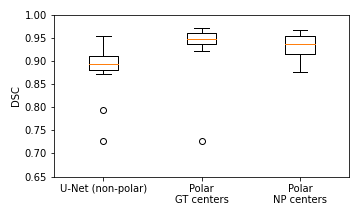
\includegraphics[width=0.6\columnwidth]{images/4/box_plot}
\caption{A box plot of the per-scan Dice coefficients of our experiments. \textit{Non-polar} are the results of the U-Net trained using cartesian images. \textit{Polar + GT centers} are the results of the U-Net trained on polar images, using ground-truth connected component centers during inference. \textit{Polar + NP centers} are the results when running inference on the polar model using center points obtained from the non-polar model predictions. \cite{bencevicUsingPolarTransform2022a}}
\label{fig:box}
\end{figure}

A comparison of our results with other deep learning-based approaches for aorta segmentation in the literature is shown in \tabref{table:comparison}. Our approach achieves performance comparable to the state of the art, and a large improvement over the baseline methods. Note that the results are evaluated on different datasets and with a different number of cases. Therefore, it is hard to objectively compare these approaches.

\begin{table}[t!]
\def\arraystretch{1.25}
\centering
\begin{tabularx}{\textwidth}{X l l c}
 \textbf{Method} & \textbf{DSC} & \textbf{mIoU} & \textbf{n}\\ 
 \hline
\citet{yuThreeDimensionalDeepConvolutional2021} & 0.958 & - & 25 \\
\citet{fantazzini3DAutomaticSegmentation2020} & $0.928 \pm 0.013$ & $0.866 \pm 0.023$ & 10 \\
\citet{cheungComputationallyEfficientApproach2021} & $0.912$ & - & 14 \\
Proposed method & $0.932 \pm 0.027$ & $0.895 \pm 0.033$ & 18 \\
\end{tabularx}
\caption{A comparison of our approach with results reported in papers describing deep learning-based aorta segmentation methods. Note that the datasets used for obtaining the results are not the same. $n$ is the number of cases used to obtain the evaluation.}
\label{table:comparison}
\end{table}

  \section{Conclusion}
    
In this chapter, we've outlined an approach to enhance data efficiency in medical image segmentation by employing two smaller neural networks, rather than a single large one. The first network is designed to predict parameters for a strategically chosen transformation, aimed at reducing the complexity of segmentation. The second network then handles the segmentation of these transformed images. Our empirical studies, particularly with the polar transform, demonstrate the efficacy of this approach across various medical imaging segmentation tasks. We observed notable improvements in training efficiency, especially in cases involving the segmentation of a single, roughly elliptical object. Furthermore, segmentation of polar-transformed images has shown state-of-the-art results in small datasets and near state-of-the-art performance in larger datasets, even when utilizing generic, low-parameter-count models such as U-Net.

We've enhanced this approach by introducing the capability to perform multiple transformations on a single image, followed by the fusion of segmentation results from each transformation using hysteresis thresholding. Applying this method using polar transformations of CT images of the aorta improved segmentation results compared to baseline networks trained on Cartesian images. This improvement was observed across various metrics without a substantial increase in training time or network architecture complexity. Moreover, the fusion of individual object segmentations on an image through hysteresis thresholding has proven beneficial in increasing pixel-level recall, a valuable trait in medical image segmentation tasks.

We have further improved this approach by allowing multiple transformations of the same image and fusing segmentations of each transformation using hysteresis thresholding. When applied to the polar transform, we showed that this leads to large improvements over baseline networks trained on cartesian images for segmenting the aorta. We see improvements across a variety of metrics without significantly increasing training times or the complexity of the used neural network architectures. In addition, by fusing separate predictions of different objects on the image with hysteresis thresholding we can increase pixel-level recall (at the cost of accuracy) which is often beneficial in medical image segmentation tasks. 

This is a flexible approach that allows leveraging domain knowledge as it can be used with any invertible image transformation. Moreover, it is invariant to the downstream segmentation architecture as it is a separate network. Thus, it can be used as a general preprocessing step regardless of the segmentation method. Moreover, if the transformation parameter predictor and segmentation networks share similar architectures, one can use transfer learning between the two networks. The approaches presented in this chapter have been published in \cite{bencevicTrainingPolarImage2021} and \cite{bencevicUsingPolarTransform2022a}.
